\documentclass[paper=letter,11pt]{scrartcl}

\KOMAoptions{headinclude=true, footinclude=false}
\KOMAoptions{DIV=14, BCOR=5mm}
\KOMAoptions{numbers=noendperiod}
\KOMAoptions{parskip=half}
\addtokomafont{disposition}{\rmfamily}
\addtokomafont{part}{\LARGE}
\addtokomafont{descriptionlabel}{\rmfamily}
%\setkomafont{pageheadfoot}{\normalsize\sffamily}
\setkomafont{pagehead}{\normalsize\rmfamily}
%\setkomafont{publishers}{\normalsize\rmfamily}
\setkomafont{caption}{\normalfont\small}
\setcapindent{0pt}
\deffootnote[1em]{1em}{1em}{\textsuperscript{\thefootnotemark}\ }


\usepackage{amsmath}
\usepackage[varg]{txfonts}
\usepackage[T1]{fontenc}
\usepackage{graphicx}
\usepackage{xcolor}
\usepackage[american]{babel}
% hyperref is needed in many places, so include it here
\usepackage{hyperref}

\usepackage{xspace}
\usepackage{multirow}
\usepackage{float}


\usepackage{braket}
\usepackage{bbm}
\usepackage{relsize}
\usepackage{tcolorbox}

\def\ketY{\ensuremath{\ket {\Psi}}}
\def\iGeV{\ensuremath{\textrm{GeV}^{-1}}}
%\def\mp{\ensuremath{m_{\textrm{proton}}}}
\def\rp{\ensuremath{r_{\textrm{proton}}}}
\def\me{\ensuremath{m_{\textrm{electron}}}}
\def\aG{\ensuremath{\alpha_G}}
\def\rAtom{\ensuremath{r_{\textrm{atom}}}}
\def\rNucl{\ensuremath{r_{\textrm{nucleus}}}}
\def\GN{\ensuremath{\textrm{G}_\textrm{N}}}
\def\ketX{\ensuremath{\ket{\vec{x}}}}
\def\ve{\ensuremath{\vec{\epsilon}}}


\def\ABCDMatrix{\ensuremath{\begin{pmatrix} A &  B  \\ C  & D \end{pmatrix}}}
\def\xyprime{\ensuremath{\begin{pmatrix} x' \\ y' \end{pmatrix}}}
\def\xyprimeT{\ensuremath{\begin{pmatrix} x' &  y' \end{pmatrix}}}
\def\xy{\ensuremath{\begin{pmatrix} x \\ y \end{pmatrix}}}
\def\xyT{\ensuremath{\begin{pmatrix} x & y \end{pmatrix}}}

\def\IMatrix{\ensuremath{\begin{pmatrix} 0 &  1  \\ -1  & 0 \end{pmatrix}}}
\def\IBoostMatrix{\ensuremath{\begin{pmatrix} 0 &  1  \\ 1  & 0 \end{pmatrix}}}
\def\JThree{\ensuremath{\begin{pmatrix}    0 & -i & 0  \\ i & 0  & 0 \\ 0 & 0 & 0 \end{pmatrix}}} 
\def\JTwo{\ensuremath{\begin{bmatrix}    0 & 0 & -i  \\ 0 & 0  & 0 \\ i & 0 & 0 \end{bmatrix}}}
\def\JOne{\ensuremath{\begin{bmatrix}    0 & 0 & 0  \\ 0 & 0  & -i \\ 0 & i & 0 \end{bmatrix}}}
\def\etamn{\ensuremath{\eta_{\mu\nu}}}
\def\Lmn{\ensuremath{\Lambda^\mu_\nu}}
\def\dmn{\ensuremath{\delta^\mu_\nu}}
\def\wmn{\ensuremath{\omega^\mu_\nu}}
\def\be{\begin{equation*}}
\def\ee{\end{equation*}}
\def\bea{\begin{eqnarray*}}
\def\eea{\end{eqnarray*}}
\def\bi{\begin{itemize}}
\def\ei{\end{itemize}}
\def\fmn{\ensuremath{F_{\mu\nu}}}
\def\fMN{\ensuremath{F^{\mu\nu}}}
\def\bc{\begin{center}}
\def\ec{\end{center}}
\def\nus{$\nu$s}

\def\adagger{\ensuremath{a_{p\sigma}^\dagger}}
\def\lineacross{\noindent\rule{\textwidth}{1pt}}

\newcommand{\multiline}[1] {
\begin{tabular} {|l}
#1
\end{tabular}
}

\newcommand{\multilineNoLine}[1] {
\begin{tabular} {l}
#1
\end{tabular}
}



\newcommand{\lineTwo}[2] {
\begin{tabular} {|l}
#1 \\
#2
\end{tabular}
}

\newcommand{\rmt}[1] {
\textrm{#1}
}


%
% Units
%
\def\m{\ensuremath{\rmt{m}}}
\def\GeV{\ensuremath{\rmt{GeV}}}
\def\pt{\ensuremath{p_\rmt{T}}}


\def\parity{\ensuremath{\mathcal{P}}}

\usepackage{cancel}
\usepackage{ mathrsfs }
\def\bigL{\ensuremath{\mathscr{L}}}

\usepackage{ dsfont }



\usepackage{fancyhdr}
\fancyhf{}


\lhead{\Large 33-444} % \hfill Introduction to Particle Physics \hfill Spring 2022}
\chead{\Large Introduction to Particle Physics} % \hfill Spring 2022}
\rhead{\Large Spring 2022} % \hfill Introduction to Particle Physics \hfill Spring 2022}

\begin{document}
\thispagestyle{fancy}

\begin{center}
{\huge \textbf{Lecture 12}}
\end{center}

{\fontsize{14}{16}\selectfont

\textbf{\underline{Relativistic Wave Equations continued}} 

Now lets do the Spin-1 case.

EM is a theory of Spin-1 interactions.

EM was the first Lorentz invariant theory.

Maxwell's Equations
\bea
\vec{\nabla} \cdot \vec{E} = \rho \hspace{1in} \vec{\nabla} \times \vec{B} - \frac{\partial\vec{E}}{\partial t} = \vec{J} \\
\vec{\nabla} \cdot \vec{B} = 0 \hspace{1in}  \vec{\nabla} \times \vec{E} - \frac{\partial\vec{B}}{\partial t} = 0
\eea
Not manifestly Lorentz Invariant.

However can put them in a LI form. 

Define $J^\mu = (\rho,\vec{J})$

Now, $\vec{E}$ and $\vec{B}$ have 6-components total.

Same number as an anti-symmetric rank two tensor: $\fmn = - F_{\nu\mu}$ :  

16 - 4 (diagonal) - 6 (lower triangle)


\be
F_{\mu\nu} = \begin{pmatrix} 0  & E_x & E_y & E_z  \\ -E_x  & 0 & -B_z & B_y \\ -E_y  & B_z & 0 & -B_x \\  -E_z  & -B_y & B_x & 0 \end{pmatrix}
\ee

This transforms under a Lorentz transformation as

\be
F_{\mu\nu} \rightarrow {\Lambda_\mu}^\rho {\Lambda_\nu}^\sigma F_{\rho\sigma}
\ee

\be
\partial_\mu \fMN = J^\nu
\ee
Is the Lorentz Invariant ``equation of Motion'' gives 2 of Maxwell's equations. 
The ``Bianchi Identity'' 
\be
\partial_\mu F_{\nu\rho} + \partial_\rho F_{\mu\nu} + \partial_\nu F_{\rho\mu}  = 0 
\ee
gives the others.

\noindent\rule{\textwidth}{1pt}

Interestingly, can also express this more simply using potentials.

eg: express E and B in terms of potentials

\be
\vec{E} = \vec{\nabla}V - \frac{\partial \vec{A}}{\partial t} \hspace{1in}  \vec{B} = \vec{\nabla} \times \vec{A}
\ee


Can use potentials defined up to ``gauge transformation''.\\
(Horrible name. Just means redefinition.) 
\be
V \rightarrow V + \frac{\partial \vec{\lambda}}{\partial t} \hspace{1in}  \vec{A} = \vec{A} + \vec{\nabla} \lambda
\ee
these give same physics for any choice of $\lambda$.

Note here there is an enormous redundancy in our description of the physics. 

OK, now lets Introduce

\be
A_\mu = (V, \vec{A}) \hspace{1in} A_\mu \rightarrow A_\mu + \partial_\mu \lambda
\ee

which allows us to write 

\be
\fmn = \partial_\mu A_\nu - \partial_\nu A_\mu
\ee
(Note that \fmn is invariant under gauge transformations.)

Gauge transformation are \underline{\underline{NOT}} deep.  
More of redundancy, not really saying anything. 

Stress that $A_\mu$ and $A_\mu + \partial_\mu \lambda$ represent the same physics state. 

Can formulate EM from Lagrangian point if using 

\be
L_{EM} = -\frac{1}{4} \fmn\fMN - J^\mu A_\mu
\ee

If the Lagrangian is both Lorentz Invariant and Gauge Invariant, the physics that follows from it will also be. 
HW: Check the gauge invariance.

\noindent\rule{\textwidth}{1pt}

Spin-1 particles that this Lagrangian describes are the photons.  
Force carriers of the electro-magnetic interaction. 

\underline{Photon equation of motion.}
Almost always most useful to think in terms of $A_\mu$ directly. 

$A_\mu$ ``photon field'' (boson) directly describes photon DoF.

Assume no sources $J_\mu$ = 0\\
Photon equation of motion is then:
\be
\partial_\mu \fMN  = 0  \Rightarrow  \partial^2 A_\mu - \partial_\mu \partial \cdot A = (\eta_{\mu\nu} \partial^2 - \partial_\mu  \partial_\nu ) A^\nu = 0
\ee


\underline{Ansatz}:
\be
A_\mu = \epsilon_\mu(p) e^{-ip\cdot x}
\ee
where $\epsilon(p)$ is  polarization vector.

eq motion $\rightarrow$ 

\bea
(\eta_{\mu\nu} \underbrace{p^2}_{=0} - p_\mu  p_\nu ) \epsilon^\nu = 0\\
\eea
or $p\cdot \epsilon = 0$

OK, with out loss of generality, can assume
\be
P = (E,0,0,E)
\ee 

Most general form of $\epsilon(p) = (a, b, c, a)$. 


Convenient to express b \& c as

\be
\epsilon_R(p) = \frac{1}{\sqrt{2}}(0,1, i,0)  \hspace{1in} \epsilon_L(p) = \frac{1}{\sqrt{2}}(0,1, -i,0)
\ee


\be
\epsilon_R \cdot \epsilon_L = -1 \hspace{1in}  {\epsilon_R}^2 = {\epsilon_L}^2 = 0
\ee

\bea
\longrightarrow P \hspace{1in} \longrightarrow P\\
\underbrace{\rightarrow}_{Spin} \hspace{1in}  \underbrace{\leftarrow}_{Spin}
\eea


What about a ? 
(Note: only expect 2 DoF form Little group) 

Gauge invariance $\Rightarrow$ a is non-physical. 


$A_\mu = 0 $ is \underline{\underline{the same}} as $A_\mu = \partial_\mu \lambda$ for any $\lambda$
(this is in the direction along $p_\mu$)

That's all for spin-1. 

\noindent\rule{\textwidth}{1pt}

OK lets back up and talk more generally now about Lagrangians. 

Unlike classically, usually don't talk about KE and PE. 

\underline{Kinetic Terms} (bi-linear - exactly two fields) \\
$\partial_\mu \phi \partial^\mu \phi$,  $\bar{\psi} \slash{\partial} \psi$, $\frac{1}{4} \fmn^2$,  ... 

\underline{Interaction Terms} (3 or more Fields)\\
$\lambda \phi^3$, $g\bar{\psi}\gamma_\mu A^\mu\psi$, $g\partial_\mu\phi A^\mu\phi$,  $gA_\mu^2A_\nu^2$, ...

\noindent\rule{\textwidth}{1pt}

How do we know which Lagrangian to use ??!?

Will start off doing a little dimensional analysis that will turn out to have shockingly large ramifications. 

We will do something very simple that is true, and turns out will skip over 40 years of massive confusion in the field (30s - 60s). 

The infinities that emerge when you actually do calculations clouded these results, turns out to all be a red herring

Correct way of thinking about it is the ``Wilsonian Way'' something called EFTs (Effective Field Theories).

There is something deep underneath that legitimises the naive answer, but it turns out the simple answer is correct. 

One of the most important things thats happened in physics in the last 50 years is understanding this deeper way of thinking about QFT.
``Will go through this, but you wont really appreciate it until you suffer the normal bad way of talking about it''


So, What are the units of the fields that we have been talking about?

\underline{Bosons}:
\be
S[\phi(t)] = \int d^4x \left[ \frac{1}{2} (\partial_\mu\phi)(\partial^\mu\phi) - \frac{m^2}{2}\phi^2      \right]
\ee
The action is dimensionless.  $e^{\textrm{iS}}$ and $d^4x$ has mass dimension = -4. $\Rightarrow \phi$ has mass dimension = 1.


So in the Lagrangian 

\bea
\int d^4x\ && \underbrace{\lambda}_{\substack{\textrm{units of $\lambda$ }\\\textrm{dimensionless}}} \Phi^4(x)         \\
         +  && \underbrace{\mu}_{\substack{\textrm{mass}\\\textrm{dimension 1}}} \Phi^3(x)         \\
         + && \underbrace{\frac{1}{M^2} \Phi^6(x) + \frac{1}{M^4} \Phi^8(x) + \frac{1}{M^2} \Phi^2(x)\partial\Phi\partial\Phi}_{\substack{\textrm{tons of things you could write down, but the}\\\textrm{vast majority of the interactions have a strength }\\\textrm{that is an inverse power of mass}}}          \\
\eea


Only a few interactions are dimensionless, or have positive mass dimension. 

\begin{itemize}
\item[]dimensionless - marginal 
\item[]positive mass dim - relevant
\item[]negative mass dim - \underline{irrelevant}
\end{itemize}


Gravity is example of Irrel interaction.  
No invariant sense of whether strong or weak: 
At low energy scale so weak that it is unimportant
At high energy scale so important that we need to change the theory (as we will see later...)

Any irrelevant theory comes equipped with a scale at which it breaks down.

In any given theory, if you want to describe physics around some fixed energy scale, all you need to know are

\begin{itemize}
\item[-] What are the particles around (fields associated with them)
\item[-] What are the possible marginal or relevant interactions between them?  Write them all down
\end{itemize}

Only a few parameters, whatever is going on at those energy scale can be accurately described by those few parameters and nothing else.

If you want to predict things very accurately them maybe you need to include the next few terms. 

Relevant terms only important at very low energies. 
Always like to think of approximation where the partilces are moving fast compared to their masses. 
In this approximation the only things that matter are the marginal interactions. 

In all cases in physics their is some \underline{physical} scale M in which your description of the physics is wrong.
(often called UV cut-off)  eg: Plank scale the whole picture is wrong. 
But if we are at energies much lower than $M_{P}$ we dont care.

Whats happening at the higher scales is encoded in the higher dim. operators.

The way to organize your thinking is scale-by-scale.

All the thinking goes into determining the interactions. 
Guaranteed to be finite number of parameters at any given scale to describe the physics accurately. 

Any theory that we write down is an effective theory. 
That is only accurate to order powers of $\frac{E}{M_\textrm{New}}$

(For us, there is something always to $\frac{E}{M_\textrm{P}}$ that we dont know, even if we understand 1 TeV, 10 - 100 TeV ... ect)

SO really we have a big tower of effective field theories each accompanied by its own cut off. 

This is the bottom-line to Wilson's  way of thinking. 

Massive restriction to the kinds of interactions that we can have and that are relevant. 

\underline{Note} incredibly different from non-relativistic QM! 
\begin{itemize}
\item[-]any crappy potential you write down (1/r ... 1/$r^{2.3}$, random linear combination ect). 
\item[-]framework itself incredibly unconstrained.
\end{itemize}

The second we put in SR+QM, 
\begin{itemize}
\item[-] dramatic kinematic things (Anti-particles / Spin-Stats) 
\item[-] the number of interactions that we are talking about are numbers we can count on our hands
\end{itemize}

In SM $\sim 19$ marginal interactions. 
Not 1, but not a continuous $\infty$, which is what you got in a NR picture of the world.

Now for a little more...

\noindent\rule{\textwidth}{1pt}

Again, think about the limit in which we can neglect the mass of all the particles, imagining high energy processes relative to the mass of the partilces

\be
= \int d^4x\ \underbrace{(\partial_\mu\phi)(\partial^\mu\phi)}_{\substack{\textrm{free theory of scalars}\\\textrm{ mass dim(Bosons) = 1}}} + \underbrace{\bar{\psi}[i\gamma_\mu\partial^\mu]\psi}_{\substack{\textrm{free theory of fermions }\\\textrm{mass dim(Fermions) = 3/2}}}
\ee

Can now write down possible interactions of dimension four. 

\be
\Phi^4 \hspace{1in} \Phi^2\partial\Phi \hspace{1in} \psi\psi\Phi
\ee 
thats it for the marginal operators.


Basic interactions in nature
\begin{figure}[h]
\centering
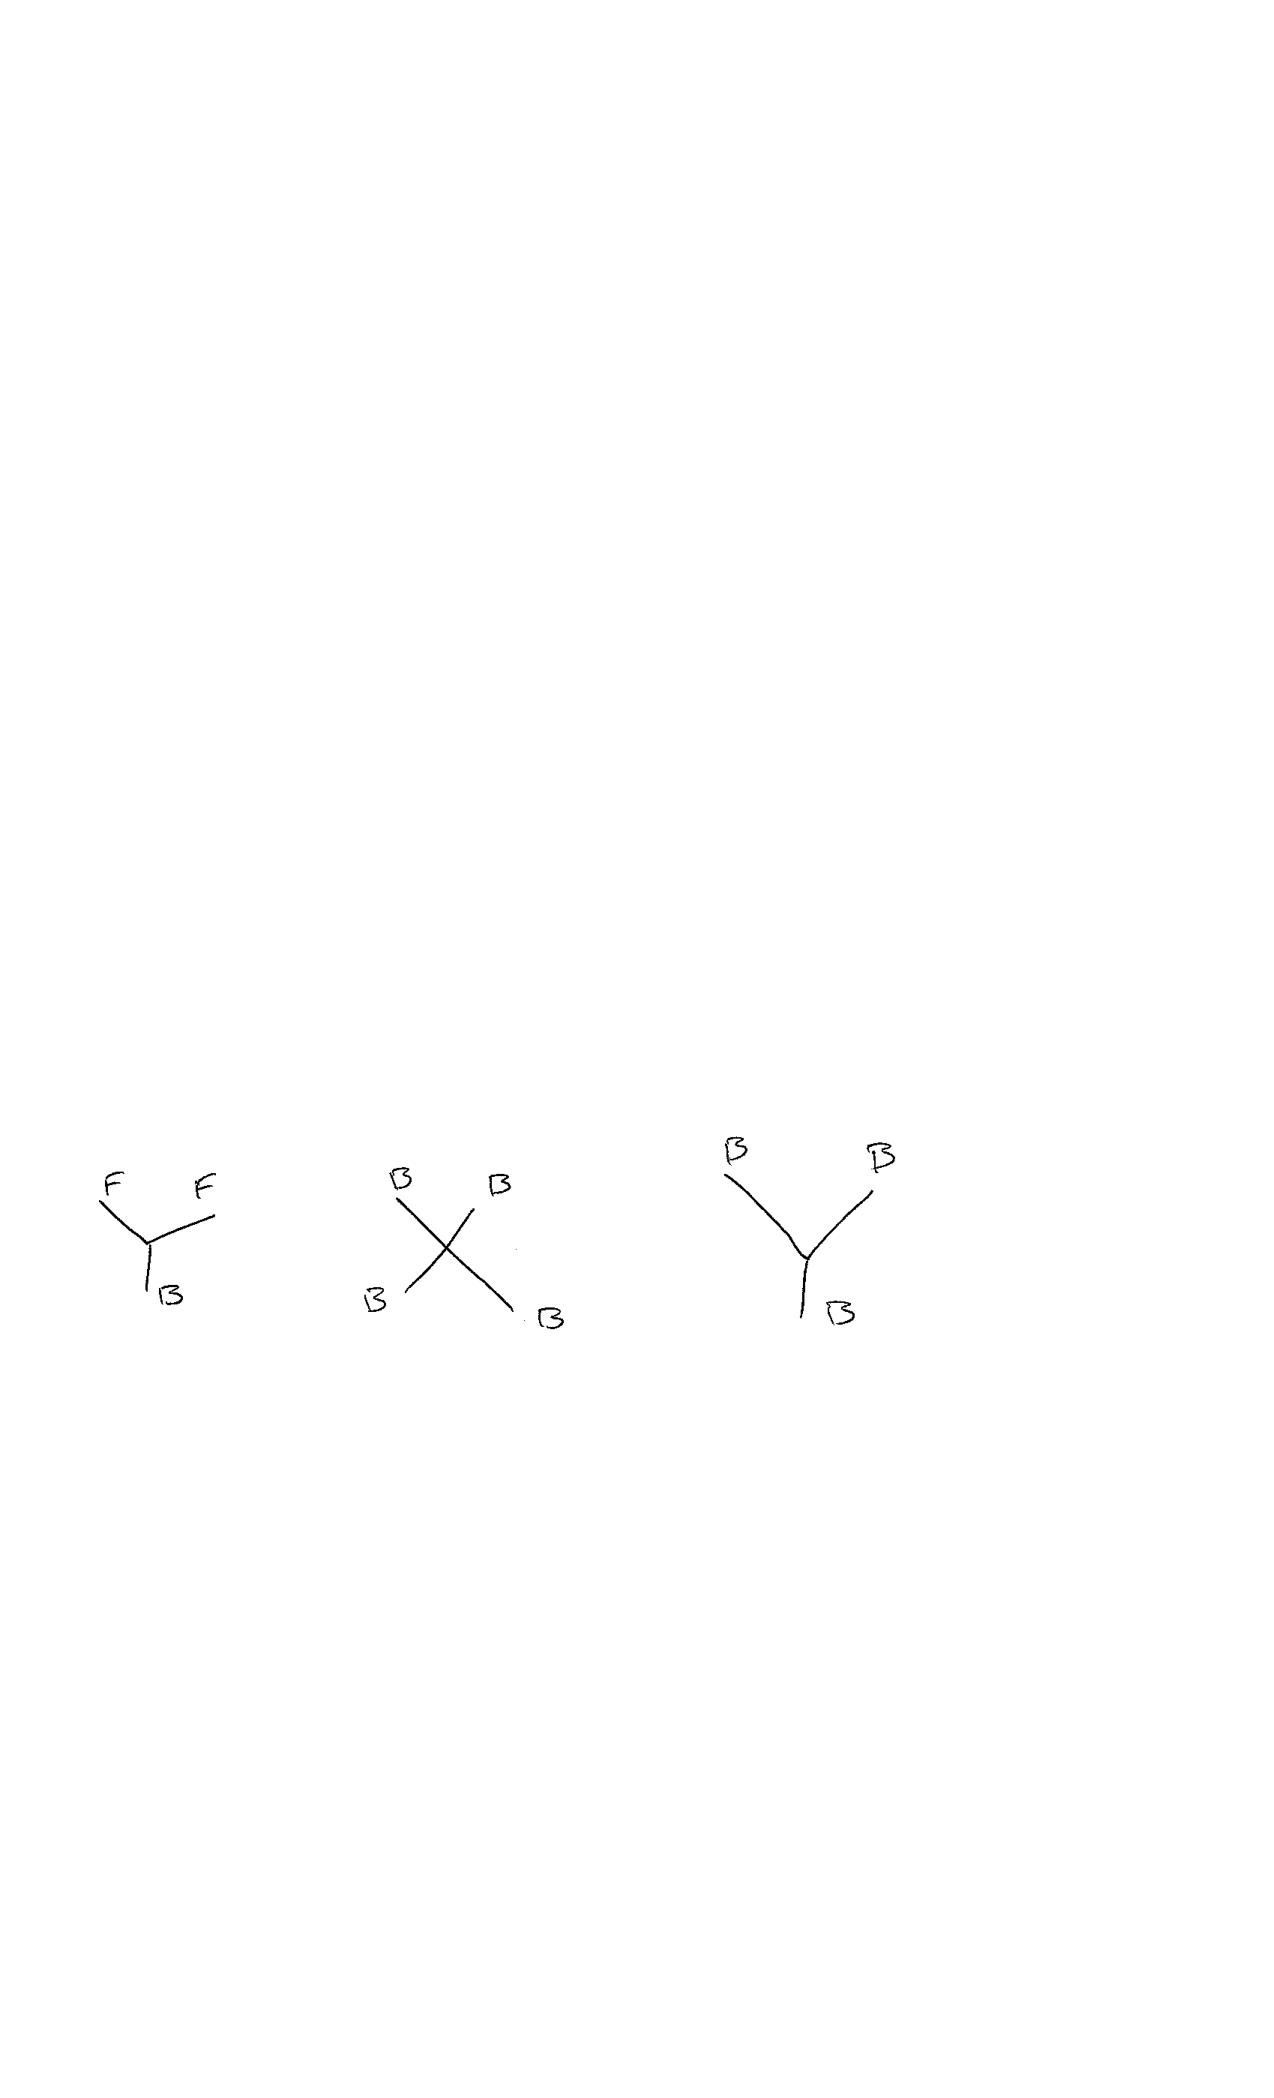
\includegraphics[width=0.9\textwidth]{./Interactions.pdf}
\end{figure}

At sufficiently low energies compared to $M_{Pl}$, SR+QM says we need a theory of Fermions \& Bosons and these are the only interactions that are important. 

Dimension counting tells us there can only be a few types of interactions, 

Next last bit of logic for why the world is such a damn constrained place...



}
\end{document}



% LocalWords:  partilces
